Tale descrizione deve contemplare almeno gli elementi riportati nelle seguenti sottosezioni.

\subsection{Convolutional neural network}

\label{sec:cnn_relu}

\emph{Descrivere in questa sezione l’architettura della convolutional neural network
sviluppata nell’ambito del progetto. Se si utilizza un’architettura nota, si riportino gli elementi fondamentali della rete e le eventuali modifiche effettuate ma, soprattutto, si motivi la scelta.
Definire in ogni caso se la rete è stata progettata come regressore (output:
numero reale da 0 a 100 che rappresenta l’età, da approssimare all’intero più
vicino) o come classificatore (output: una delle 101 classi da 0 a 100) e fornire dettagli e motivazioni sulla funzione di costo scelta.}

L'architettura scelta è MobileNetV3 Large \cite{mobilenetv3}. Le reti neurali convoluzionali (CNNs) MobileNet sono conosciute per essere progettate pensando all'applicazione su sistemi mobili e/o embedded, cercando un trade-off tra prestazioni e risorse computazionali richieste. Hanno introdotto tecniche che migliorano l'efficienza, come la \emph{depthwise separable convolution} (MobileNetV1), i \emph{linear bottleneck} e la \emph{inverted residual structure} (MobileNetV2), la \emph{squeeze and excitation} (ResNet) e le funzioni di attivazione \emph{swish}. MobileNetV3, nelle sue versioni Small e Large, è il risultato di una combinazione di questi blocchi, ottimizzata tramite \emph{platform-aware NAS} e l'algoritmo \emph{NetAdapt} \cite{mobilenetv3}. 

Per essere efficiente, MobileNetV3 presenta un numero ridotto di pesi da addestrare rispetto ad altre architetture della letteratura, e ciò l'ha resa un ottimo candidato per l'addestramento con le risorse limitate di Google Colab (VRAM e 12 ore di tempo macchina). A parità di tempo, ci è possibile addestrare la rete su più immagini, quindi è possibile utilizzare un dataset estremamente ricco di campioni che, secondo i risultati di \cite{miviaage}, garantisce ottime prestazioni anche a reti più leggere.

Il nostro modello è una versione personalizzata dell'implementazione di MobileNetV3 Large sul framework Keras\footnote{\url{https://www.tensorflow.org/api_docs/python/tf/keras/applications/MobileNetV3Large}}. In questa nostra versione distinguiamo il \emph{bottom}, cioè i livelli più bassi, quelli che svolgono le operazioni di estrazione delle feature dall'input, ed il \emph{top}, cioè gli ultimi sei livelli della rete, che producono l'output finale sulla base della feature estratte ai livelli inferiori. Per quanto riguarda la input size, l'abbiamo fissata a $224 \times 224$, mentre per quanto riguarda l'output abbiamo adattato il modello per diventare un regressore, sostituendo il top per la classificazione con un top di output unitario con attivazione Rectified Linear Unit (ReLU). Questo ci ha permesso di astrarci dalla rappresentazione dell'età, in modo da lasciarla definita nell'intervallo \([0, +\infty)\), e di utilizzare la ben nota in letteratura Mean Squared Error (MSE) loss function
\begin{displaymath}
\text{MSE} = \frac{1}{n} \sum_{i=1}^{n} \left(Y_i - \hat{Y}_i\right),
\end{displaymath}
che tiene conto anche dell'entità della differenza tra la stima dell'età e la \emph{ground truth}.

Si noti infine che nel model summary visualizzato dalla nostra implementazione il terzultimo livello viene denominato \emph{Logits}. Si tratta semplicemente del nome che l'implementazione sulla quale ci siamo basati dà al livello precedente a quello di output, ma non ha nulla a che vedere con la funzione matematica logit\footnote{\url{https://github.com/tensorflow/tensorflow/blob/v2.4.0/tensorflow/python/keras/applications/mobilenet_v3.py}, alla definizione della classe MobileNetV3, riga 312}.

\subsection{Procedura di addestramento}
\subsubsection{Dataset}
\label{subsubsec:dataset}

Il dataset utilizzato per addestrare la nostra rete a compiere il task assegnato è il dataset chiamato \emph{VGG-Face2 Mivia Age}, anche detto \emph{VMAGE}\cite{miviaage}.

Quest'ultimo dataset contiene $3.067.620$ immagini di $8921$ soggetti. Ad ogni immagine è associata l'età del soggetto, tale valore è una stima dell'età apparente del soggetto catturato.
Il dataset ci è stato fornito già diviso in training set, che include $8.421$ identità, e test set, che include le rimanenti $500$.

Le risorse che \textit{Google Colab} mette a disposizione sono risultate insufficienti per allenare la rete sull'intero training set, pertanto è stato necessario ridurre la grandezza di quest'ultimo. A tale scopo è stata svolta un analisi del training set e sono stati scelte le identità sulle quali svolgere l'addestramento della rete. Tale analisi è stata svolta combinando le annotazioni per VMAGE riguardanti la sola età con annotazioniper VGGFace2\footnote{Tali annotazioni sono reperibili al seguente link: \url{https://github.com/MiviaLab/GenderRecognitionFramework/releases/tag/0}} contenenti, tra le altre, informazioni riguardanti il genere e il numero di sample per ogni identità e, per ogni immagine, la regione dell'immagine contenente il volto del soggetto ivi rappresentato, che è stata utilizzata per svolgere operazioni dettagliate più avanti.

Appurato quindi che era necessario ridurre il numero di campioni, ci siamo chiesti se vi fosse qualche sbilanciamento all'interno del dataset che potevamo mitigare durante il nostro processo di eliminazione di dati. Abbiamo pertanto svolto una prima analisi sul genere delle identità presenti.

\begin{figure}[ht]

\begin{subfigure}{0.5\textwidth}
\def\svgscale{0.5}
\input{./Images/gender_ids.pdf_tex}
\caption{Identità divise per genere}
\label{sfig:Ids per gender}
\end{subfigure}
\begin{subfigure}{0.5\textwidth}
\def\svgscale{0.5}
\input{./Images/gender_images.pdf_tex}
\caption{Immagini divise per genere}
\label{sfig:Images per gender}
\end{subfigure}
\caption{Divisione per genere di identità e immagini}
\label{fig:gender_division}
\end{figure}

Come possiamo vedere in figura~\ref{sfig:Ids per gender} e \ref{sfig:Images per gender}, il training set risulta sbilanciato in favore degli uomini per quanto riguarda il genere dei soggetti.

Successivamente abbiamo analizzato, per ogni identità, la \emph{media} e la \emph{deviazione standard} delle età ad essa associate.

\begin{figure}[ht]

\begin{subfigure}{0.5\textwidth}
\def\svgscale{0.42}
\input{./Images/n_ids_by_age_and_gender.pdf_tex}
\caption{Identità divise per genere ed età media}
\label{sfig:Ids per gender and mean age}
\end{subfigure}
\begin{subfigure}{0.5\textwidth}
\def\svgscale{0.42}
\input{./Images/n_images_by_age_and_gender.pdf_tex}
\caption{Immagini divise per genere ed età media}
\label{sfig:Images per gender and mean age}
\end{subfigure}
\caption{Divisione per genere di identità e immagini}
\label{fig:gender_age_division}
\end{figure}

Come si evince dai grafici in figura~\ref{sfig:Ids per gender and mean age} e in figura~\ref{sfig:Images per gender and mean age}, ci sono delle fasce d'età sovrarappresentate rispetto alle altre, in particolare le fasce d'età $[25,34]$ e $[35,44]$.

Abbiamo quindi scelto di escludere dal set le identità relative a uomini nelle fasce $[25,34]$ e $[35,44]$, e quelle relative a donne nella fascia $[25,34]$. In entrambi i casi abbiamo rimosso soltanto identità per le quali la deviazione standard dell'età risulta inferiore a $5.5$, per un totale di $3249$ identità. Il risultato di tale operazione è visibile in figura~\ref{fig:Ids per gender and mean age after the drop}.

\begin{figure}[ht]
\centering
\def\svgscale{0.7}
\input{./Images/n_ids_by_age_and_gender_after_drop.pdf_tex}
\caption{Identità divise per genere ed età media dopo il taglio}
\label{fig:Ids per gender and mean age after the drop}
\end{figure}

Successivamente a tale operazione, al training set sono state sottratte ulteriori $480$ identità, scelte casualmente, che hanno formato il \emph{validation set}. La tecnica di validazione utilizzata consiste quindi nell'approccio training e validation set \emph{vanilla}, quindi senza l'utilizzo di approcci tipo \emph{cross-validation} e simili, in quanto troppo esose dal punto di vista computazionale.

In conclusione:
\begin{itemize}
	\item Il training set è composto da $4692$ identità per un totale di $1.68$ milioni di immagini;
	\item Il validation set è composto da $480$ identità per un totale di $170363$ immagini;
	\item Il test set è composto da $500$ identità per un totale di $169372$ immagini.
\end{itemize}
\subsubsection{Face detection}
\label{subsubsec:face_detection}

\emph{Descrivere il metodo utilizzato per effettuare il rilevamento del volto. Se si utilizza un approccio noto o i volti già estratti con framework esistenti, si specifichi questa informazione.}

Per il rilevamento del volto non abbiamo utilizzato un face detector, in quanto nelle annotazioni del dataset VGGFace2, già citate nel paragrafo~\ref{subsubsec:dataset}, sono riportate sia per il training set che per il test set, informazioni inerenti alle bounding boxes relative ai volti dei soggetti immortalati. Tali informazioni definiscono quindi la \textbf{region of interest} (ROI) di ogni immagine.
Ovviamente, qualora questa rete dovesse essere utilizzata per un'applicazione reale, andrebbe aggiunto un face detector a monte del sistema di age estimation.

Ad esempio, per ricavare le annotazioni da noi utilizzate è stato utilizzato un face detector basato su una versione di \emph{SSD} che usa ResNet-10 come rete backbone \cite{miviagender}.

\subsubsection{Face pre-processing} 

\emph{Descrivere e motivare tutte le tecniche di pre-processing applicate sulle immagini del volto.}

Il pre-processing è stato suddiviso per semplicità in due fasi. La prima fase precede quella di data augmentation, e consiste nel ritaglio del volto del soggetto. Il ritaglio viene effettuato su di una regione individuata dalla ROI(paragrafo~\ref{subsubsec:face_detection}) allargata di un fattore $0.3$ \cite{vggface2dataset}, ovviamente non andando oltre i limiti dettati dalla risoluzione dell'immagine. Tale operazione permette di ritagliare oltre al volto del soggetto l'intera testa. Questa operazione viene effettuata prima della data augmentation perché alcune operazioni lì implementate modificano la posizione del volto all'interno dell'immagine, e quindi le ROI risulterebbero invalide. Tuttavia, qualora il sistema di age estimation dovesse essere utilizzato insieme ad un face detector, quest'ultimo dovrebbe ricevere in input le immagini già sottoposte ad augmentation, in quanto questa tecnica mira ad introdurre nel dataset modifiche dell'immagine più o meno tipiche del mondo reale, che si presenterebbero sull'immagine prima che questa possa essere sottoposta a rilevamento del volto.

Nella seconda fase di pre-processing, che viene effettuata a valle della data augmentation, ogni immagine viene ridimensionata alla dimensione di input della rete, e viene eseguita anche una normalizzazione. 

Nel caso in cui l'immagine necessiti di essere ingrandita verrà effettuato un sovracampionamento con interpolazione cubica, in quanto questo algoritmo garantisce ottimi risultati, pur presentando una complessità computazionale non eccessiva. In particolare, una delle caratteristiche dell'interpolazione cubica che risulta particolarmente adatta al nostro dataset, considerato che in esso vi sono molte immagini aventi risoluzione inferiore all'input size della rete, è l'assenza di pixelation nell'output.
Nel caso in cui, invece, l'immagine dovesse essere sottocampionata, verrà utilizzata un'interpolazione lineare. 

In entrambi i casi, il ridimensionamento viene effettuato mantenendo le proporzioni originali dell'immagine, e nel caso in cui l'immagine ritagliata non fosse quadrata viene aggiunto del padding. 

Dopo le operazioni di ridimensionamento, ad ogni immagine viene sottratta la media, per ogni canale, delle immagini del dataset VGGFace. Ciò permette alla distribuzione degli input di essere centrata in $0$, permettendoci di sfruttare tutti i vantaggi della non linearità della ReLu (paragrafo~\ref{sec:cnn_relu}) ed ottenere una convergenza più veloce \cite{miviaage}.

\begin{figure}[ht]
\centering
\begin{subfigure}{0.3\textwidth}
\includegraphics[width=\textwidth]{./Images/detection.jpg}
\caption{ROI evidenziata per quest'immagine}
\label{sfig:detection}
\end{subfigure}
\hspace{0.1\textwidth}
\begin{subfigure}{0.3\textwidth}
\includegraphics[width=\textwidth]{./Images/preprocessed.jpg}
\caption{Il risultato del ritaglio}
\label{sfig:preprocessed}
\end{subfigure}
\caption{Preprocessing a monte della data augmentation}
\label{fig:preprocessing}
\end{figure}

\subsubsection{Data augmentation}
\emph{Descrivere e motivare tutte le policy di augmentation implementate per estendere il dataset o per aumentarne la rappresentatività.}
Per la data augmentation, durante l'addestramento applichiamo una serie di filtri in maniera casuale. Non essendo stato formulato uno use-case specifico per il sistema, lo scopo della fase di data augmentation è quello di aumentare la rappresentatività del training set, con modifiche dell'immagine tipiche del setting di acquisizione del nostro dataset (come indicato nel paragrafo~\ref{sec:intro.intention}), oltre che a fornire resilienza ad attacchi basilari. Questa fase è stata implementata senza aumentare la cardinalità del dataset, considerato che questo è già sufficientemente grande.

I filtri applicati sono:
\begin{enumerate*}[label={\alph*)}]
\item \emph{rumore gaussiano additivo} con media 0 e deviazione standard nell'intervallo $[0.08, 0.15]$, come prevenzione ad attacchi semplici che sfruttano questo effetto ed anche per tenere in conto il rumore introdotto dal sensore fotografico;
\item \emph{blur gaussiano} con deviazione standard nell'intervallo $[1, 2.5]$, presente soprattutto in immagini di cui si fa un sovracampionamento tramite filtro bicubico o in immagini con errori di messa a fuoco;
\item \emph{ritaglio} \cite{miviagender}, per cui l'immagine viene tagliata ulteriormente per simulare fotografie in cui la faccia non è ripresa completamente o errori del face detector;
\item \emph{rotazione} nell'intervallo $[-10 \degree, 10 \degree ]$, \item \emph{rovesciamento} rispetto all'asse verticale e \item \emph{inclinazione} \cite{miviagender} nello spazio tridimensionale per rendere la rete invariante rispetto all'inclinazione/orientamento del volto all'interno dell'immagine;
\item \emph{spatter} \cite{miviagender}, ossia schizzi e macchie per rendere la rete invariante rispetto a possibili coperture del viso, sia digitali che volontarie;
\item \emph{variazione di luminosità} nell'intervallo $[-50\%, -10\%] \cup [10\%, 50\%]$ e \item \emph{variazione di contrasto} nell'intervallo $[0.1, 0.4] \cup [1.5, 5.0]$, per l'invarianza rispetto a condizioni di luce diverse.
\end{enumerate*}
Per ogni immagine, viene scelto casualmente se applicare o meno un filtro. In caso positivo, viene scelto casualmente uno dei filtri insieme ad un valore di intensità che ricada nell'intervallo predisposto per ognuno di essi.

Gli intervalli all'interno dei quali viene scelta l'intensità di applicazione di ogni filtro sono uguali a quelli presenti nelle implementazioni del Mivia Gender Recognition Framework \cite{miviagender}, eventualmente personalizzati, secondo i valori esplicitamente indicati, sulla base di alcune prove effettuate manualmente.
I valori scelti empiricamente fanno sì che l'effetto dell'applicazione del filtro non sia completamente distruttivo e il risultato sia ancora riconoscibile all'occhio umano rispetto all'immagine originale.

\begin{figure}[ht]
\begin{subfigure}[t]{0.18\textwidth}
\includegraphics[width=\textwidth]{./Images/preprocessed.jpg}
\caption{Nessun effetto applicato}
\label{sfig:corruption_contrast}
\end{subfigure}\hfill
\begin{subfigure}[t]{0.18\textwidth}
\includegraphics[width=\textwidth]{./Images/contrast_severity_0.2.jpg}
\caption{Contrasto aumentato di $0.2$}
\label{sfig:corruption_contrast}
\end{subfigure}\hfill
\begin{subfigure}[t]{0.18\textwidth}
\includegraphics[width=\textwidth]{./Images/brightness_severity_-0.3.jpg}
\caption{Luminosità ridotta del $30\%$}
\label{sfig:corruption_brightness}
\end{subfigure}\hfill
\begin{subfigure}[t]{0.18\textwidth}
\includegraphics[width=\textwidth]{./Images/gaussian_blur_severity_2.0.jpg}
\caption{Blur gaussiana con deviazione standard $0.2$}
\label{sfig:corruption_gaussian_blur}
\end{subfigure}\hfill
\begin{subfigure}[t]{0.18\textwidth}
\includegraphics[width=\textwidth]{./Images/gaussian_noise_severity_0.1.jpg}
\caption{Rumore gaussiano con deviazione standard $0.1$}
\label{sfig:corruption_gaussian_noise}
\end{subfigure}\hfill

\begin{subfigure}[t]{0.18\textwidth}
\includegraphics[width=\textwidth]{./Images/horizontal_flip.jpg}
\caption{rovesciamento rispetto all’asse verticale}
\label{sfig:corruption_skew}
\end{subfigure}\hfill
\begin{subfigure}[t]{0.18\textwidth}
\includegraphics[width=\textwidth]{./Images/skew.jpg}
\caption{inclinazione nello spazio tridimensionale}
\label{sfig:corruption_skew}
\end{subfigure}\hfill
\begin{subfigure}[t]{0.18\textwidth}
\includegraphics[width=\textwidth]{./Images/spatter_severity_3.jpg}
\caption{Spatter con severità $3.0$}
\label{sfig:corruption_spatter}
\end{subfigure}\hfill
\begin{subfigure}[t]{0.18\textwidth}
\includegraphics[width=\textwidth]{./Images/random_crop_severity_0.3.jpg}
\caption{Ritaglio del $30\%$}
\label{sfig:corruption_random_crop}
\end{subfigure}\hfill
\begin{subfigure}[t]{0.18\textwidth}
\includegraphics[width=\textwidth]{./Images/rotation_severity_7.0.jpg}
\caption{Rotazione di $7.0 \degree$}
\label{sfig:corruption_rotation}
\end{subfigure}\hfill
\caption{Possibili applicazioni dei filtri}
\label{sfig:data_augmentation}
\end{figure}

\subsubsection{Training from scratch o fine tuning}
\emph{Specificare se la rete viene addestrata con inizializzazione random o partendo da pesi pre-addestrati, motivando la scelta e fornendo dettagli sulla strategia di inizializzazione.}

Come già precisato nel paragrafo~\ref{sec:cnn_relu}, come base per il nostro addestramento abbiamo realizzato una versione di MobileNetV3Large basata su di un'implementazione già disponibile in Keras. 

Abbiamo inizializzato il \emph{bottom} con pesi appresi su ImageNet\cite{imagenet}, mentre per quanto riguarda il \emph{top} abbiamo inizializzato l'unico livello che richiede pesi, quello convoluzionale, in maniera randomica. In particolare, per questo livello abbiamo lasciato l'inizializzazione di default prevista dall'implementazione, ovvero l'inizializzazione uniforme di Glorot, sebbene di solito si preferisca l'inizializzazione uniforme di He per layer con funzione d'attivazione ReLU\todo{aggiornare quando scegliamo modello definitivo}, in quanto le due inizializzazioni differiscono soltanto per un fattore al numeratore della varianza della distribuzione utilizzata (1 in Glorot, 2 in He), ed il fatto di non cambiare l'inizializzazione ci ha permesso di non dover modificare l'implementazione della rete (ovviamente, se la rete avesse prodotto risultati diversi da quelli attesi, saremmo ritornati anche su questo punto).

Abbiamo scelto di seguire questa strada in quanto il fatto di partire da pesi appresi su di un dataset generico e molto vasto permette di ridurre i tempi di convergenza dell'algoritmo di addestramento\cite{miviaage}. 

Ovviamente non abbiamo potuto riutilizzare i pesi ImageNet per il \emph{top} della rete, in quanto ImageNet è un dataset tipicamente utilizzato per la classificazione.

\subsubsection{Procedura di training}
\todo{Indicare probabilità di corruzioni e probabilità di corruzioni frequenti, batch size.}
\emph{Dettagliare e motivare almeno le seguenti scelte: numero di epoche di addestramento, tipo di ottimizzatore, learning rate scheduling (tecnica di riduzione, learning rate iniziale, fattore di riduzione). Fornire dettagli su eventuali elementi aggiuntivi: batch normalization, weight decay, early stopping etc. Per ognuna delle scelte, riportare i valori esatti dei parametri utilizzati, per rendere l’esperimento riproducibile. Motivare la scelta di tali valori.}

\begin{comment}
	- Learning rate OK
		- Scheduling: a quali epoche l'abbiamo ridotto e perché
		- Warmup: come l'abbiamo fatto, perché (citare paper)
		- Come l'abbiamo ridotto, quando, fattore di riduzione
	- Ottimizzatore OK
		- Perché Adam (magari citare paper)
		- Parametri, perché dei valori
	- Regolarizzazione OK
		- No weight decay
		- Batch normalizatin forse è inclusa in mobilenet
	- Perché abbiamo levato di mezzo early stopping (forse) OK
	- Numero di epoche OK
		- Ci siamo basati sul MAE. Avremmo potuto ripartire da capo e cambiare learning rate prima, ma non abbiamo avuto tempo.
\end{comment}

È stato scelto Adam \cite{adam} perché in molti casi offre prestazioni paragonabili a SGD richiedendo meno operazioni di tuning dei parametri. In particolare gestisce i momenti in maniera adattiva e rende le implementazioni "classiche" del weight decay poco incisive. Tutto ciò ci ha permesso di ridurre il numero di tentativi (e quindi il tempo) necessari a trovare una buona configurazione dell'ottimizzatore. Difatti, l'algoritmo ci ha richiesto soltanto di intervenire in diminuzione sul learning rate quando le metriche monitorate non miglioravano significativamente. 
Per quanto riguarda gli altri parametri, i valori di default riportati in \cite{adam} e forniti dall'implementazione Keras di Adam sono risultati ottimali.

Infine, Adam offre il vantaggio non indifferente dell'avere learning rate adattivi per ogni peso della rete.

Per ciò che concerne le tecniche di regolarizzazione, MobileNetV3 include all'uopo livelli di batch normalization e dropout. Non abbiamo messo in atto strategie di weight decay perché gli approcci "classici" a questa tecnica (in pratica quelli basati su regolarizzazione $L_2$) sono poco efficaci con Adam \cite{adam_no_wd} e visti i risultati sul validation set non ci è sembrato necessario approfondire ulteriormente l'argomento. 

PROCEDURA DI TRAINING IN GENERALE (learning rate, numero di epoche etc.)
Infine, per quanto riguarda il learning rate, abbiamo eseguito 2000\cite{adam_warmup} step di warmup, partendo con un learning rate pari 0 ed incrementandolo fino a raggiungere il valore di default previsto per Adam, cioè $0.001$. Successivamente, abbiamo ridotto il learning rate di un fattore 20 in tre momenti diversi:
\begin{itemize}
	\item dopo l'epoca 6, in quanto la fase oscillatoria sul validation set della loss e del MAE era terminata ed abbiamo avuto valori paragonabili di queste metriche per due epoche consecutive; possiamo notare come successivamente a questa diminuzione vi sia una sostanziale riduzione dei valori assunti da entrambe le funzioni;
	\item dopo l'epoca 12, perché il MSE e il MAE avevano ripreso ad oscillare, seppur in un intervallo particolarmente ridotto;
	\item dopo l'epoca 16, perché le metriche si erano praticamente stabilizzate sui nuovi valori, e volevamo verificare se vi fosse ancora margine di miglioramento.
\end{itemize}
Avevamo anche predisposto delle callback per la riduzione automatica del learning rate e per l'early stopping, tuttavia abbiamo scelto di non utilizzarle perché l'osservazione diretta delle curve ci ha permesso maggiore controllo. Questi strumenti potrebbero essere impiegati dopo questo primo esperimento per un eventuale addestramento sull'intero training set.

La rete è stata allenata per un totale di $19$ epoche, tuttavia scegliamo come modello definitivo quello all'epoca XX, in quanto le epoche successive non hanno apportato miglioramenti significativi alle metriche osservate. \todo{mettere numero vero di epoca alla quale ci fermiamo}

\begin{figure}[ht]
	\centering
	\hfill
	\begin{subfigure}[b]{0.47\textwidth}
		\centering
		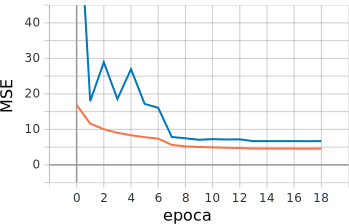
\includegraphics[width=\textwidth]{epoch_loss}
	\end{subfigure}
	\hfill
	\begin{subfigure}[b]{0.47\textwidth}
		\centering
		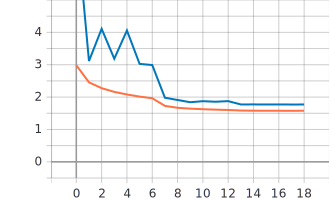
\includegraphics[width=\textwidth]{epoch_mae}
	\end{subfigure}
	\hfill
	\caption{Andamento delle metriche durante l'addestramento.}
\end{figure}
